\documentclass[a4paper,11pt]{article}
\usepackage{amsmath}
\usepackage{graphicx}
\usepackage{caption}
\usepackage{amssymb}
\usepackage{verbatim}
\usepackage{hyperref}
\usepackage{listings}
\usepackage{float}
\usepackage[thinc]{esdiff}
\usepackage{euscript}
\usepackage{subcaption}
\usepackage{enumitem}
\usepackage{commath}
\setlength{\parindent}{0em}
\newcommand*{\field}[1]{\mathbb{#1}}%
\usepackage{amsthm}
\newtheorem{claim}{Claim}
\captionsetup{labelformat=empty}
\usepackage[nottoc]{tocbibind}
\usepackage{adjustbox}



\begin{document}
\lstset{language = Matlab}
\begin{titlepage} % Suppresses displaying the page number on the title page and the subsequent page counts as page 1
	
	\center % Centre everything on the page
	
	\vspace*{3cm}

	\textsc{Mathematical Tripos, Part II}\\
	\textsc{Computational project}
	\begin{center}
      {\huge\bfseries Phase and group velocity\\[0.4cm]
}     \end{center}
	
	\vfill
	\vfill\vfill\vfill\vfill
	\includegraphics*[width = 2.675cm, height = 3.1cm]{coat.png}
	\vfill
    \textsc{University of Cambridge}
	
	\vspace*{\fill}
	\vfill
	{\large\today} 
	\vfill
	
\end{titlepage}
\setcounter{tocdepth}{3}
\tableofcontents
\newpage
\section{Question 1}
The Klein-Gordon equation is:
\begin{equation}
u_{tt} - c_0^2 u_{xx} = -q^2 u
\label{1}
\end{equation}
with $c_0 > 0$ and $q > 0$ constants.
The initial values are: 
\begin{equation}
u(x,0) = f(x),\; u_t (x,0) = 0
\label{2}
\end{equation}
We can set $c_{0} = 1$ without lost of generosity because we may rescale the Klein-Gordon equation by $x \to c_0x$. \\
Substitute the Fourier Transform 
$$
u(x,t) = \Re\left(\frac{1}{2 \pi} \int_{-\infty}^{\infty}
\tilde{u}(k,t) e^{ikx} dk \right)
$$
into \ref{1}, we have
$$\tilde{u}_{tt}+(q^2+k^2) \tilde{u} = 0$$
which hints on a separation of variables $\tilde{u}(k,t) = \tilde{X}(k)T(t)$ and $\tilde{X}(k) = \tilde{f}(k)$. Then the equation becomes an ODE for T. One solution of the ODE is $T(t) = e^{-i\Omega(k)t}$, where $\Omega(k) = \sqrt{q^2+k^2}$, which is even in k.\\
We now verify that 
\begin{equation}
u(x,t)  = \Re\left(\frac{1}{2\pi} \int_{-\infty}^{\infty} \tilde{f}(k)e^{i(kx-\Omega(k)t)}dk\right)
\label{3}
\end{equation}
is exactly a solution subject to the initial conditions \ref{2}. The first condition is satisfied trivially. For the second condition, we need to make some observations.\\
Note that f is real and even in x, $\tilde{f}$ is real and even in k. We also know that $\Omega(k)$ is even in k, hence $\int_{-\infty}^{\infty} \Omega(k)\tilde{f}(k)\sin(kx)dk  = 0$. 
Therefore, since 
\begin{align*}
u_t (x,0)  &= -\Re\left(\frac{1}{2\pi} \int_{-\infty}^{\infty} i\Omega(k)\tilde{f}(k)e^{ikx}dk\right)\\
&= \frac{1}{2\pi}\int_{-\infty}^{\infty} \Omega(k)\tilde{f}(k)\sin(kx)dk = 0,
\end{align*}
\ref{3} is a solution of the K-G equation \ref{1} subject to ICs \ref{2}.
\begin{figure}[H]
 \center
 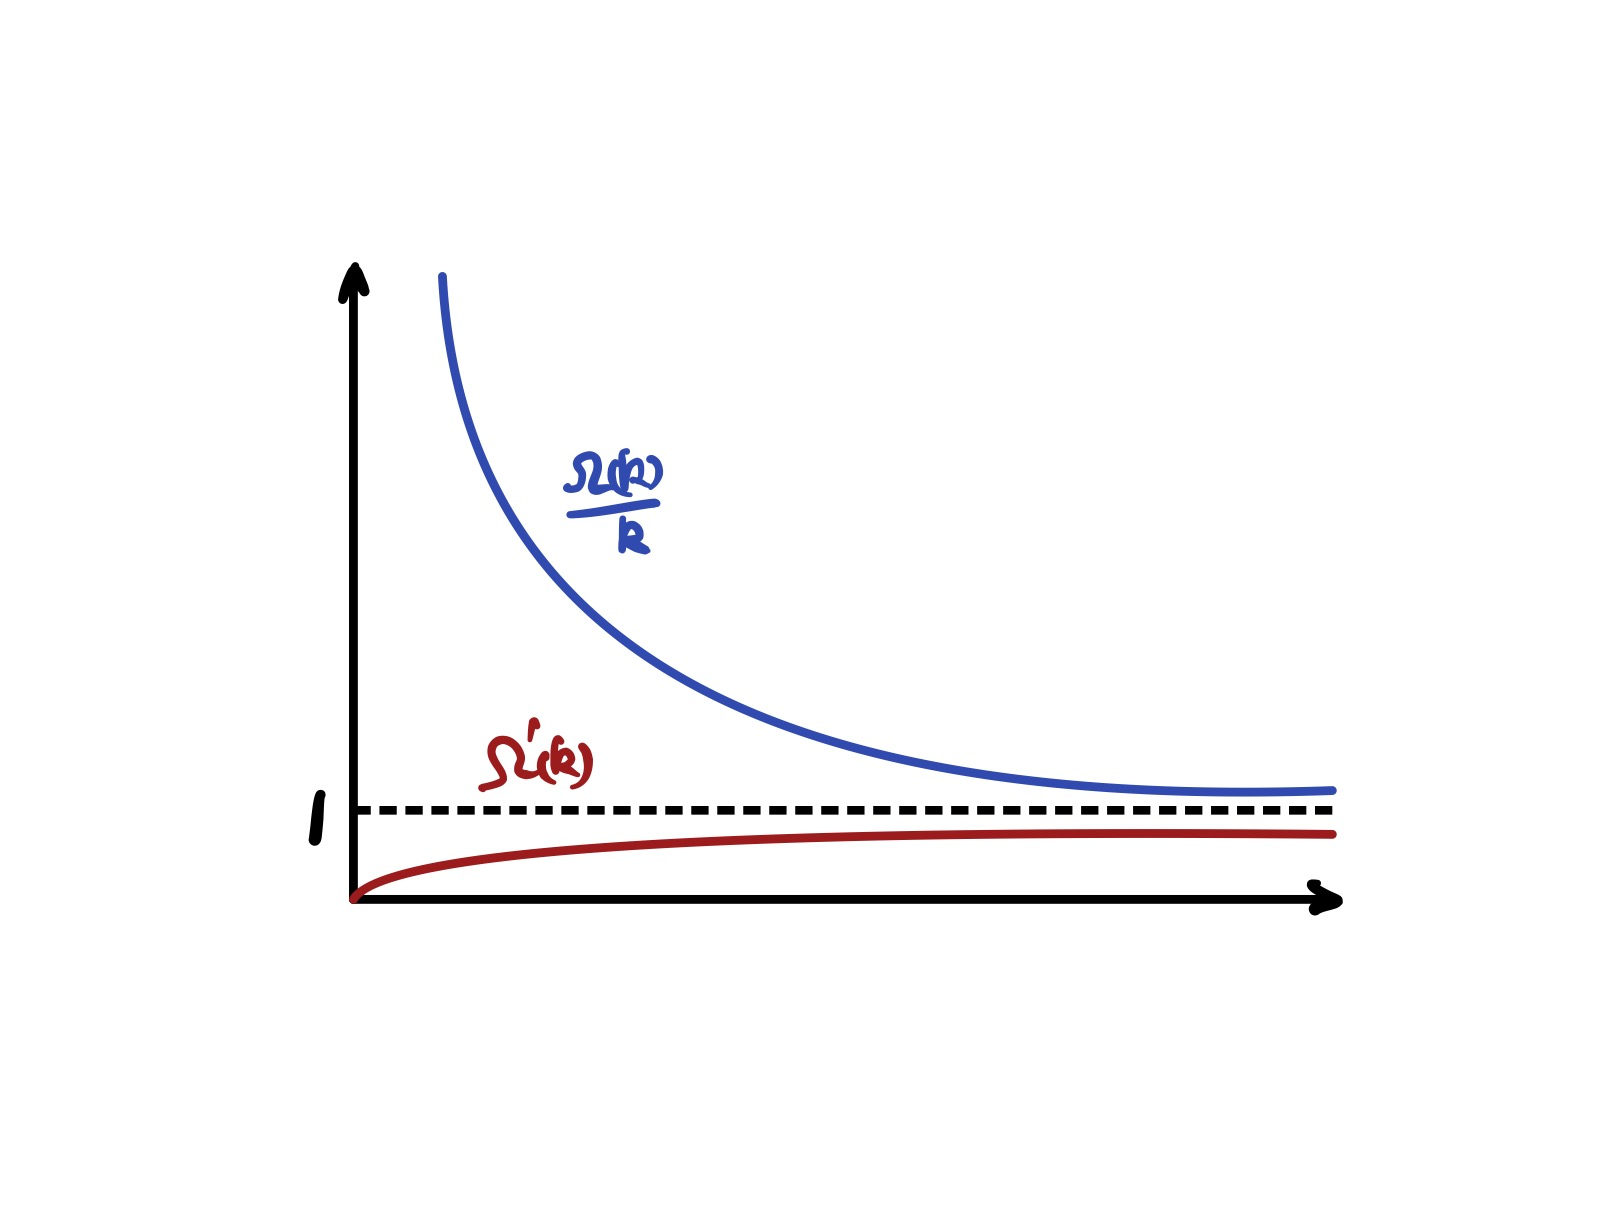
\includegraphics[width = 0.9\linewidth, height =8cm]{Q1.jpg}
 \caption{Figure 1: Characteristics of step-like Initial data}
 \label{Q1}
\end{figure}
The figure 1 is the graph of phase velocity $c_p (k)\frac{\Omega(k)}{k}$ and group velocity $c_g (k)\Omega'(k)$ against k. The phase velocity $c_p (k)$ is the travelling velocity of the crests of the wave with wave number k. 
\section{Question 2}
\subsection*{The method of stationary phase}
For a Fourier integral of the type $$\varphi (x,t) = \int_{-\infty}^{\infty}F(k)e^{i(kx-\Omega(k)t)}dk$$, we are interested in the behaviour for both large x and large t. A particular choice of $V = x/t$ allows us to examine waves moving with the velocity. We can write $\chi(k) = \Omega(k) - kx/t$, and the integral is written $$\varphi (x,t) = \int_{-\infty}^{\infty}F(k)e^{-i\chi(k)t}dk.$$ For large t the main contribution to the integral is from a small neighbourhood of the stationary points of $\chi(k)$. 
\\
\\
Use the method of stationary phase, for fixed $V = x/t$, the phase of \ref{3} is given by $$\chi(k) = \Omega(k) - kV,$$ which has stationary points $k_0$ such that $ \Omega'(k_0) = V.$ and $$k_0 = \frac{Vq}{\sqrt{1-V^2}}$$.
Expand $\chi$ and $\tilde{f}$ in Taylor series at $k = k_0$, the dominant terms are
\begin{align*}
\tilde{f}(k) &\sim \tilde{f}(k_0)\\
\chi(k) &\sim \chi(k_0) + \frac{(k-k_0)^2}{2} \chi''(k_0)
\end{align*}
Therefore, 
$$
u(x,t) \sim \Re \left((2\pi)^{-1}\tilde{f}(k_0)e^{-i\chi(k_0)t}\int_{k_0-\epsilon}^{k_0+\epsilon} e^{-\frac{i}{2} (k-k_0)^2 \chi''(k_0)t}dk\right). 
$$
By using a change of variable $s = \sqrt{\frac{|\chi''(k_0)|t}{2}}(k-k_0)$
$$
 \sim \Re\left((2\pi)^{-1}\tilde{f}(k_0)e^{-i\chi(k_0)t}\sqrt{\frac{2}{|\chi''(k_0)|t}}\int_{k_0-\epsilon}^{k_0+\epsilon} e^{-is^2}ds\right) 
$$
It can be verified from integration by parts that the contributions not from
 stationary points $\sim \mathcal{O}(1/t)$ as $t\to \infty$. Hence
$$
 \sim \Re\left((2\pi)^{-1}\tilde{f}(k_0)e^{-i\chi(k_0)t}\sqrt{\frac{2}{|\chi''(k_0)|t}}\int_{-\infty}^{\infty} e^{-is^2}ds\right) 
$$
By Cauchy's theorem and Jordan's lemma, we can deform the contour of integration to $z(r) = re^{-\frac{\pi i}{4}}$. \\

Therefore 
\begin{align*}
& \sim \Re\left((2\pi)^{-1}\tilde{f}(k_0)e^{-i\chi(k_0)t}\sqrt{\frac{2}{|\chi''(k_0)|t}}e^{-\frac{\pi i}{4}} \int_{-\infty}^{\infty} e^{-x^2}dx\right)
\\
& \sim \Re\left([2\pi|\chi''(k_0)|t]^{-\frac{1}{2}}\tilde{f}(k_0) e^{-i(\chi(k_0)t+\frac{\pi}{4}})\right)
\end{align*}
By $\chi''(k_0) = \Omega''(k_0) = q^{-1}(1-V^2)^{3/2}$ and $\tilde{f}(k_0) = |\tilde{f}(k_0)|e^{i(\arg\tilde{f}(k_0))}$, and the fact that $|V| < 1$,
\begin{align*}
&\sim \Re\left([2\pi|\Omega''(k_0)|t]^{-\frac{1}{2}}|\tilde{f}(k_0)| e^{-i(\chi(k_0)t-\arg\tilde{f}(k_0)+\frac{\pi}{4})}\right)\\
\text{and}\\
 u(x,t)& \sim [2\pi \Omega''(k_0) t]^{-\frac{1}{2}}|\tilde{f}(k_0)| \cos(k_0 x - \Omega(k_0)t+\arg\tilde{f}(k_0)-\frac{\pi}{4})
\end{align*}
Then by direct substitution, write in terms of x, t, with the condition $|V| < 1$ replaced by  $|x|<t$,
\begin{equation}
u(x,t) \sim \frac{q^{1/2}t}{(2\pi)^{1/2}(t^2-x^2)^{3/4}}\tilde{f}\left(\frac{qx}{\sqrt{t^2-x^2}}\right)\cos\left(q\sqrt{t^2-x^2}+\frac{1}{4}\pi\right)
\label{4}
\end{equation}
We observe that V is the group velocity at wave number $k_0$. When the observer travels at the group velocity $\Omega'(k)$, as $t\to \infty$, the leading contribution comes from the corresponding wave number and the contributions from all other wave numbers goes to zero. As a result, the wave number is conserved with the group velocity. \\ Therefore, the \textbf{information} carried forward by a wave travels at the group velocity. 
\section{Question 3}
The programme can be found in the \ref{P1}.\\
The reason for setting $u_i^{-1} = u_i^{1}$ is that we have the initial condition $u_t(x,0) = 0$. 
\begin{figure}[H]
 \begin{subfigure}{0.5\textwidth}
 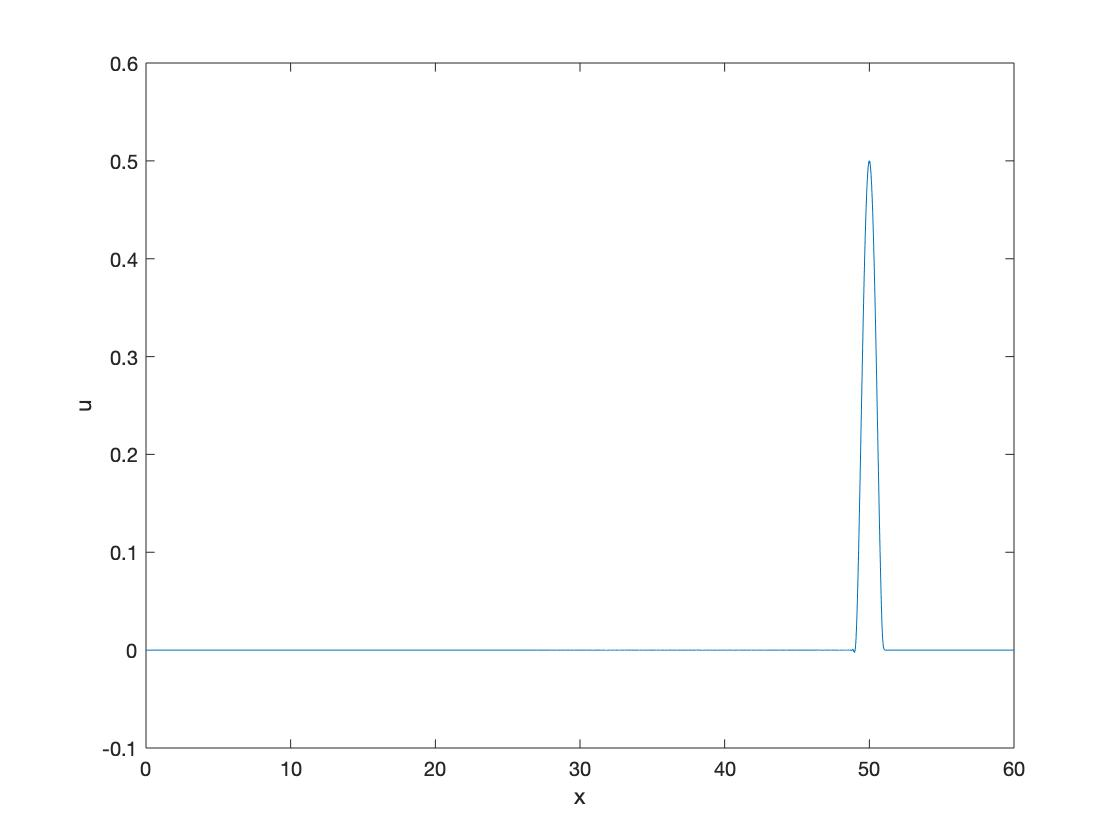
\includegraphics[width = \linewidth, height =5cm]{Q3.jpg}
 \caption{Numerical solution of Klein-Gordon  equation at q = 0}
 \label{Q3}
 \end{subfigure}
  \begin{subfigure}{0.5\textwidth}
 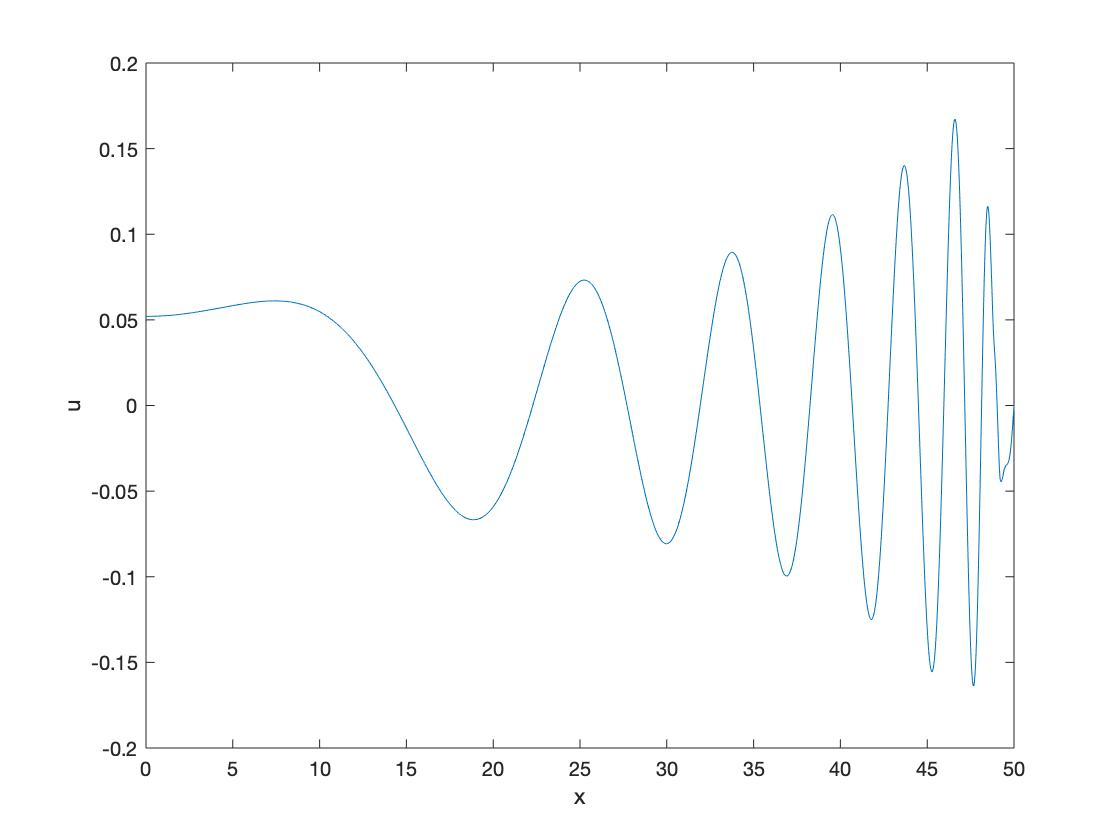
\includegraphics[width = \linewidth, height =5cm]{Q3(c).jpg}
 \caption{Numerical solution of Klein-Gordon equation at q = 1}
 \label{Q3(1)}
 \end{subfigure}
 \caption{Figure 3.2}
\end{figure} 
A few experiments were carried out for different values of k and k/h. It turns out that the scheme could become unstable for a large value of k. \\
We do a Fourier stability analysis: 
$$\hat{u}^{n+1}(\theta) = -\hat{u}^{n-1}(\theta) + 2\left(1-\frac{k^2}{h^2}+\cos\theta\left(\frac{1}{h^2}-\frac{q^2}{2}\right)\right)\hat{u}^{n}(\theta)$$
The characteristic equation is quadratic. The product of the roots is 1, therefore stability (that requires the moduli of both $\lambda$ to be at most one) is equivalent to the roots being complex conjugate, so we require (for all $\theta \in [-\pi, \pi)$)
$$\left(1-\frac{k^2}{h^2}+(1-2\sin^2 \frac{\theta}{2})\left(\frac{1}{h^2}-\frac{q^2}{2}\right)\right)^2\leqslant 1$$
Therefore, as long as our choices for k and h satisfy the above inequality the scheme is stable. 
By substituting the exact solution into the numerical scheme, the local truncation error is $\mathcal{O}(h^2+k^2)$.
\begin{figure}[H]
 \begin{subfigure}{0.5\textwidth}
 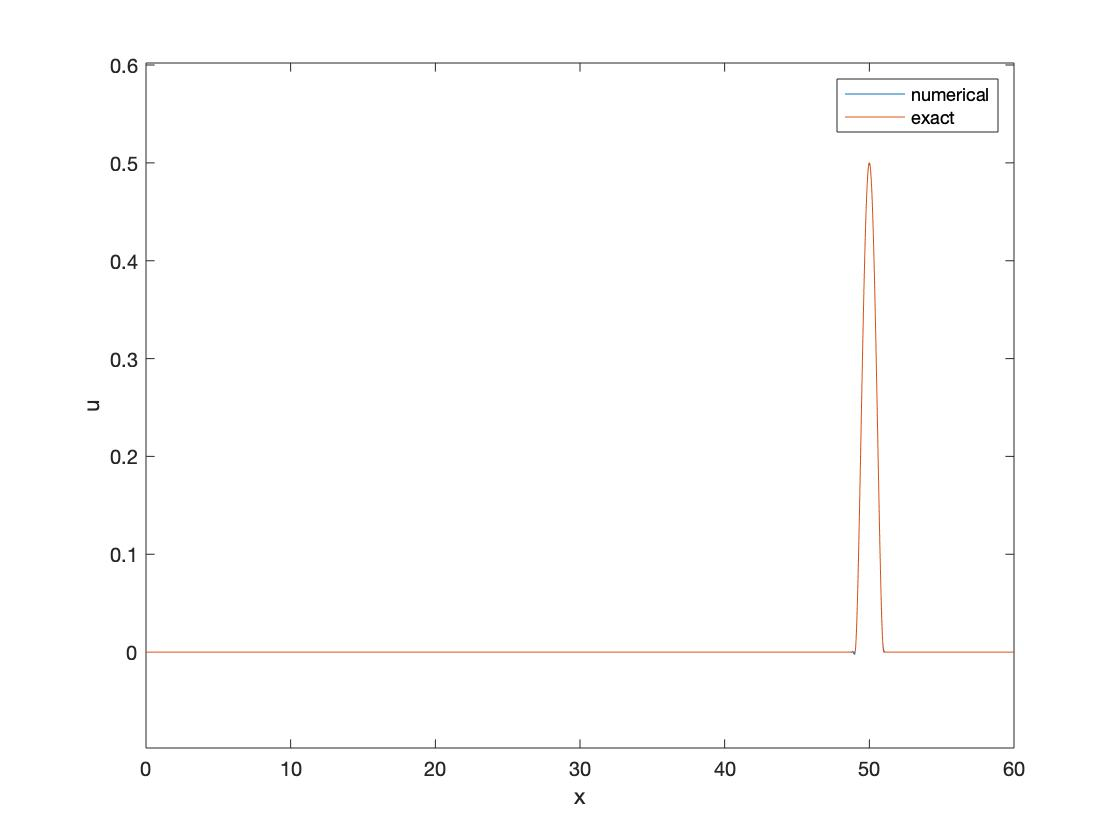
\includegraphics[width = \linewidth, height =5cm]{Q3(i).jpg}
 \caption{Numerical and exact solution of wave equation at t = 50}
 \label{Q3(a)}
 \end{subfigure}
  \begin{subfigure}{0.5\textwidth}
 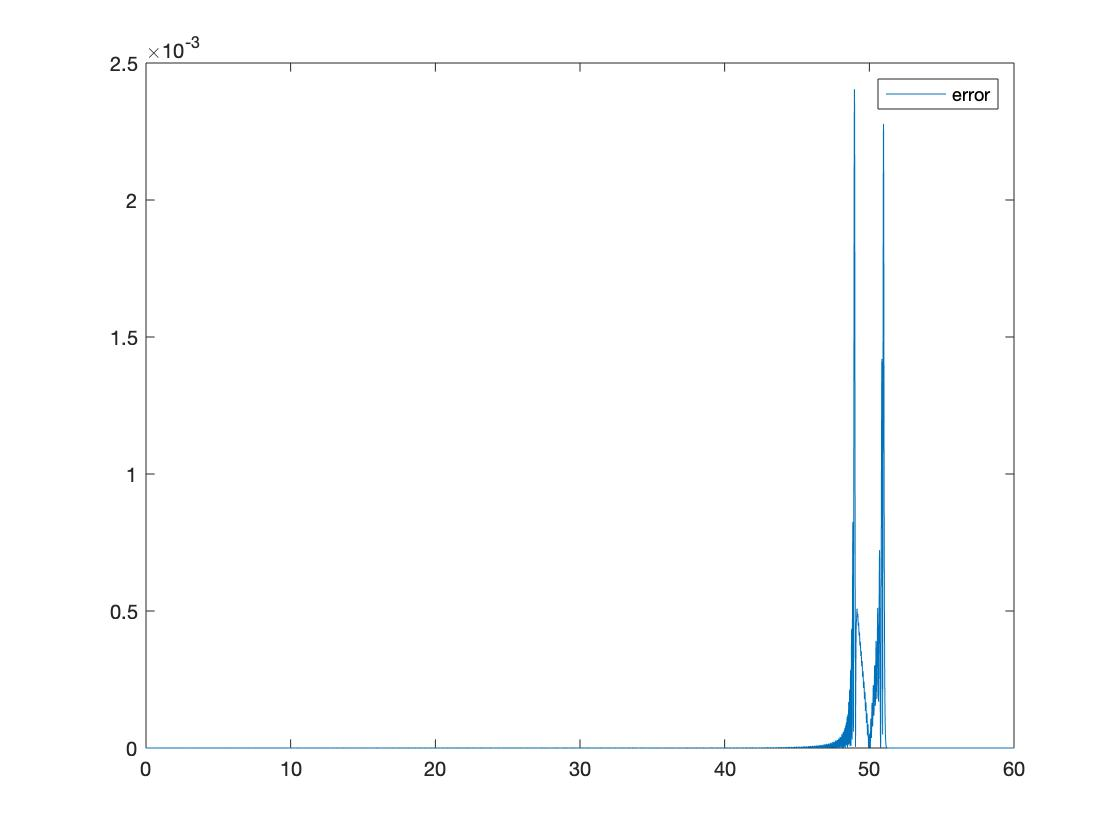
\includegraphics[width = \linewidth, height =5cm]{Q3(ii).jpg}
 \caption{Error\\at t = 50, x = 60}
 \label{Q3(b)}
 \end{subfigure}
 \caption{Figure 3.2}
\end{figure}

The Fourier Transform of the initial condition is
$$\tilde{f}(k) = -\frac{16((k^2-3)\sin k)+3k\cos k)}{k^5}.$$
\begin{figure}[H]
 \center
 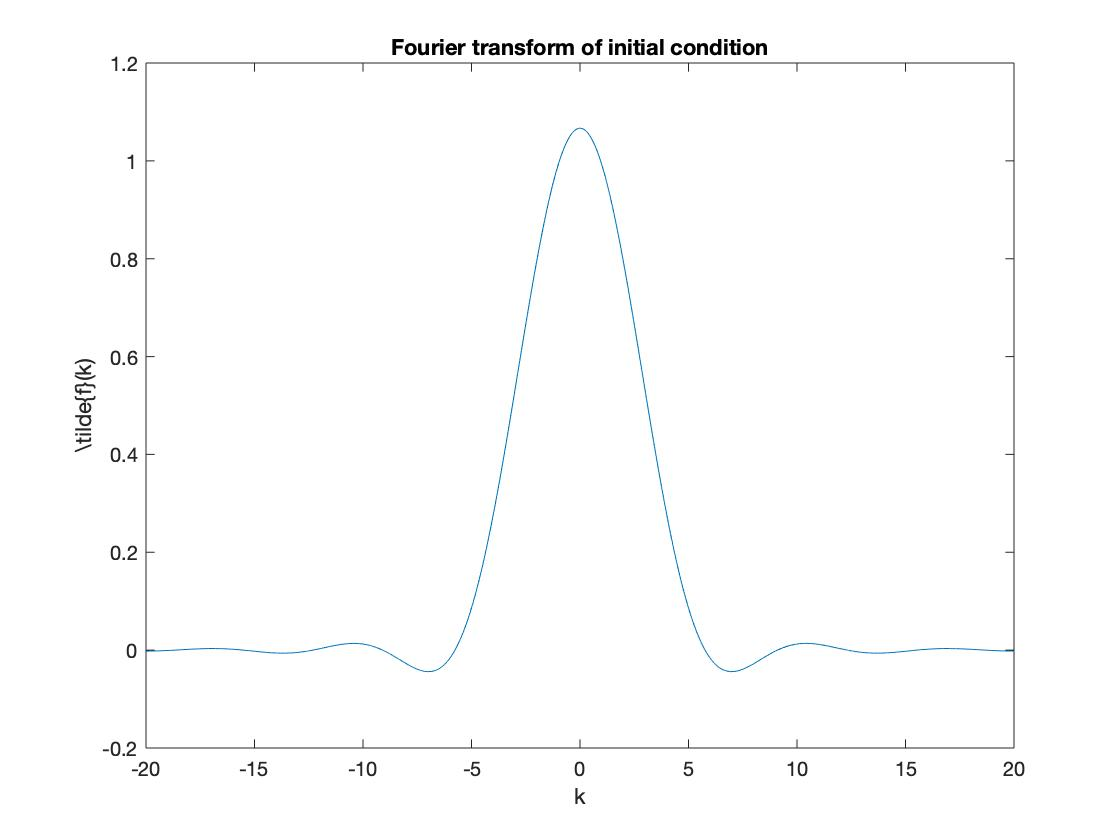
\includegraphics[width = 0.5\linewidth, height =5cm]{Q3(2).jpg}
 \caption{Figure 3.3: Fourier Transform of the initial condition}
 \label{Q3(2)}
\end{figure}
Then we plot the finite-difference solutions of case q = 1 at various times. For the case q = 1, we superpose the stationary-phase approximation. 
\begin{figure}[H]
 \begin{subfigure}{0.5\textwidth}
 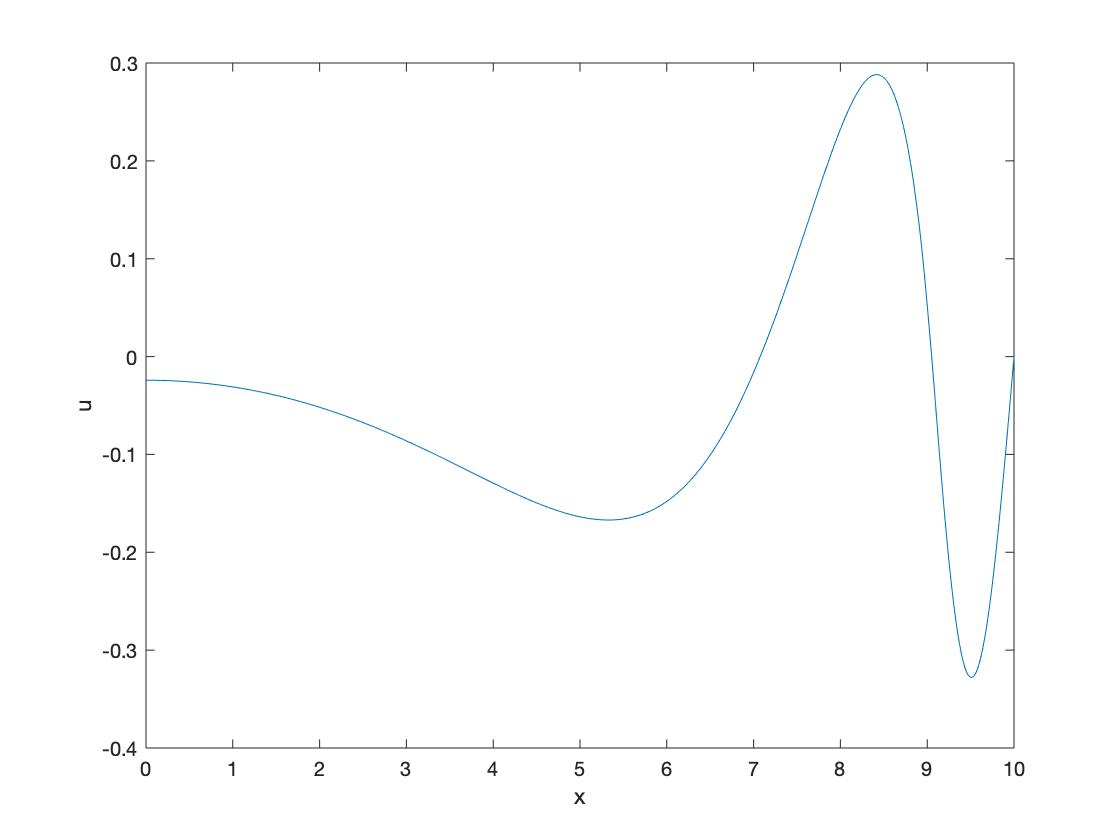
\includegraphics[width = \linewidth, height =5cm]{Q3(a).jpg}
 \caption{Numerical solution of \\Klein-Gordon equation at q = 1 \\when t = 10}
 \label{Q3(a)}
 \end{subfigure}
  \begin{subfigure}{0.5\textwidth}
 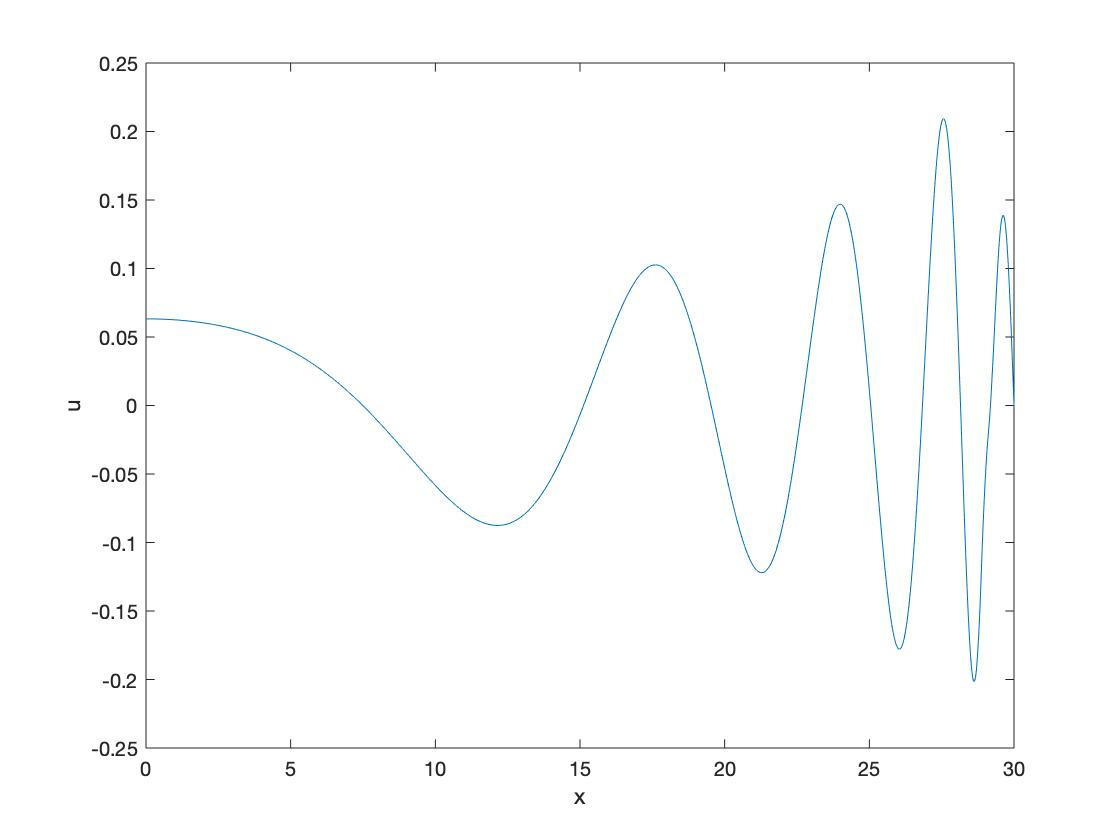
\includegraphics[width = \linewidth, height =5cm]{Q3(b).jpg}
 \caption{Numerical solution of \\Klein-Gordon equation at q = 1 \\when t = 30}
 \label{Q3(b)}
 \end{subfigure}
 \begin{subfigure}{0.5\textwidth}
 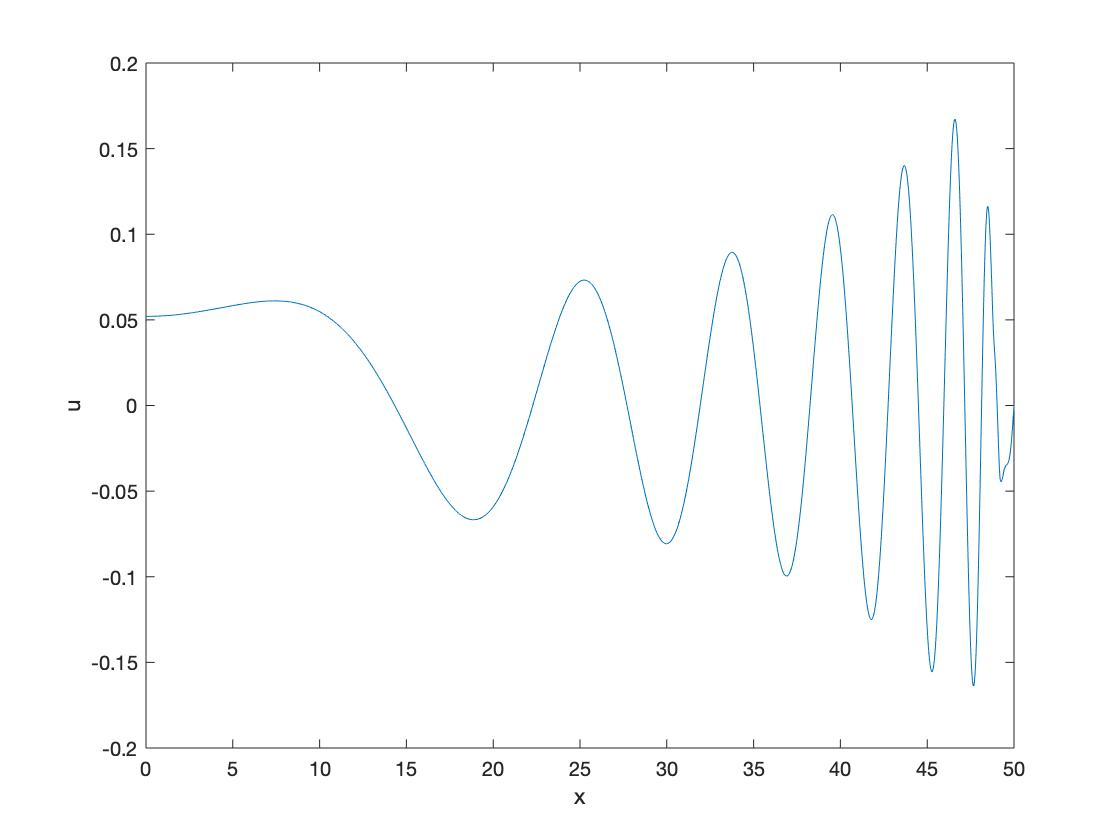
\includegraphics[width = \linewidth, height =5cm]{Q3(c).jpg}
 \caption{Numerical solution of \\Klein-Gordon equation at q = 1 \\when t = 50}
 \label{Q3(c)}
 \end{subfigure}
 \begin{subfigure}{0.5\textwidth}
 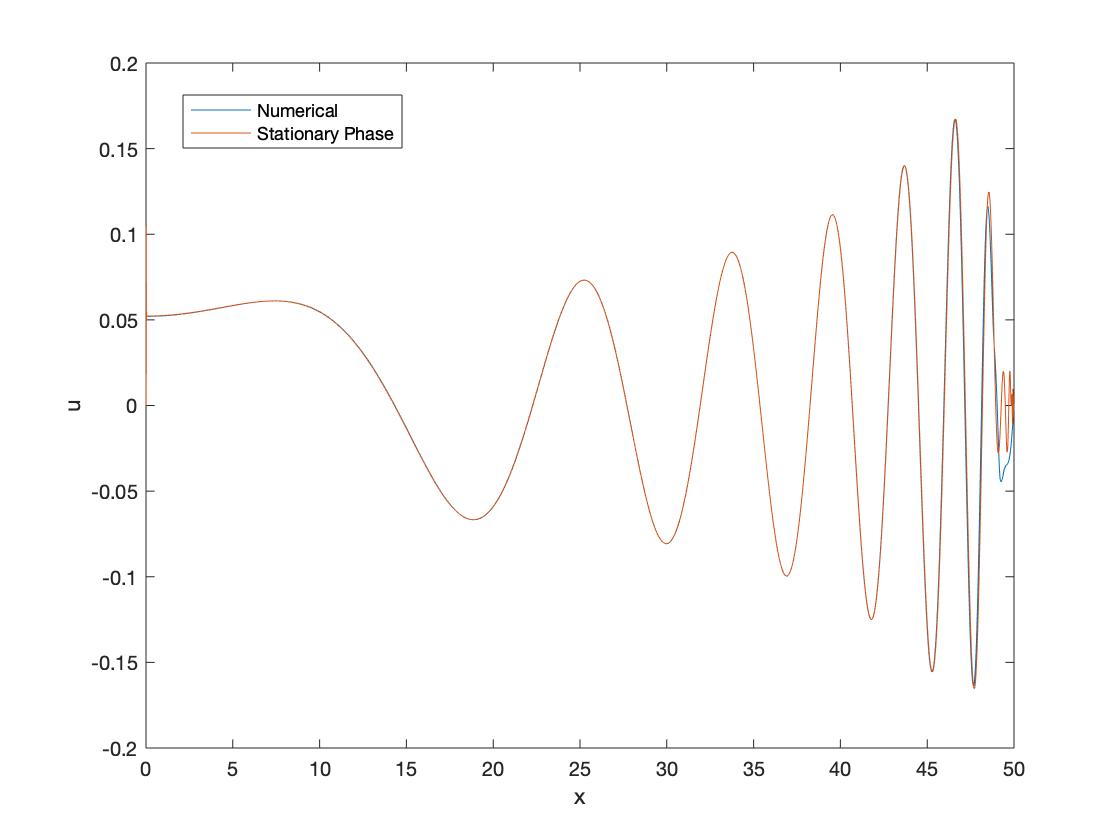
\includegraphics[width = \linewidth, height =5cm]{Q3(3).jpg}
 \caption{Numerical Solution and \\Stationary-Phase approximation \\ at t = 50.}
 \label{Q3(3)}
 \end{subfigure} 
 \caption{Figure 3.4}
\end{figure}
There is a right travelling wave solution for both q = 0 and q = 1.However, for q = 0 there is a solitary wave solution, while for q = 1 there is a train of peaks and troughs. If q is positive and very small, one would expect the amplitude of one peak much greater than those of the others, which are close to zero.
\section{Question 4}
When q = 0, $u(x,t) = 0$ by d'Alembert's solution. In this problem we assume that there is a signal $u(0,t) = \sin(\omega_0 t)$ at the left boundary, so the second initial condition $u_t(x,0)$ is dropped, and we expect a travelling wave solution $\frac{1}{2}(\sin\omega_0 (t-x)+\sin\omega_0(t+x))$
\begin{figure}[H]
\begin{subfigure}{0.5\textwidth}
 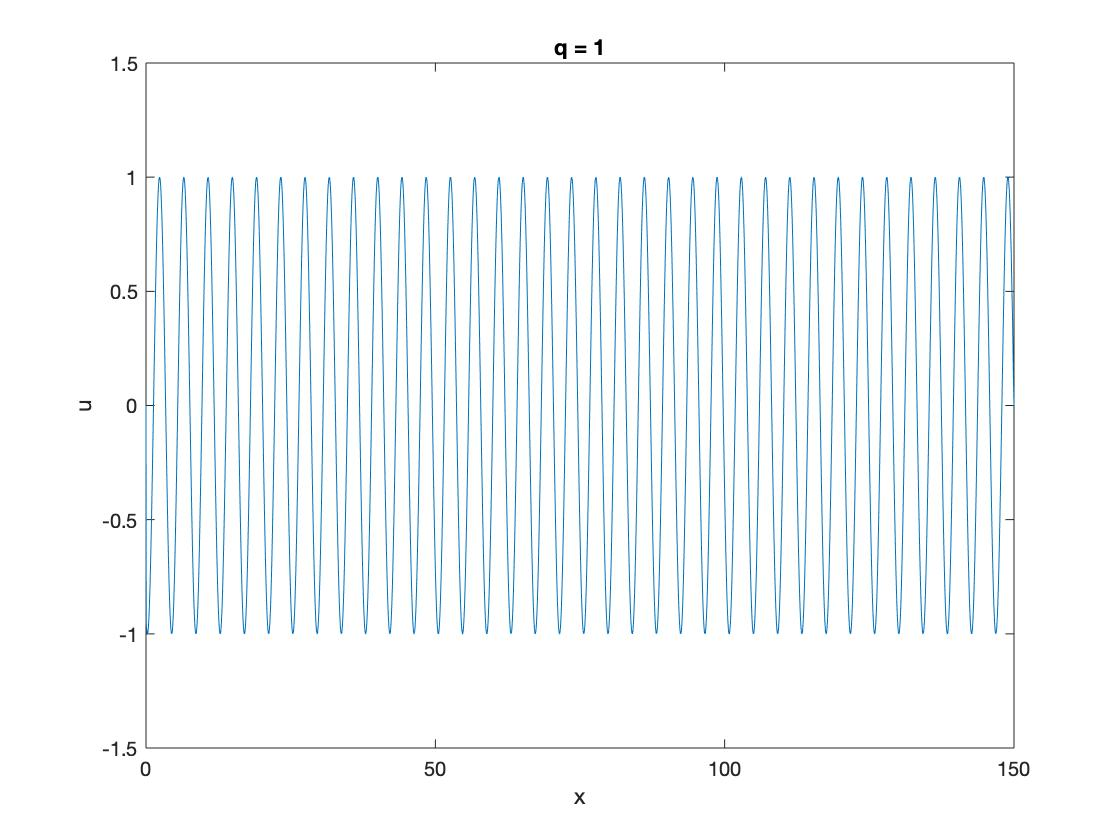
\includegraphics[width = \linewidth, height =5cm]{Q4(0).jpg}
 \caption{Signal when q = 0, $\omega = 1.5$, \\at t = 150}
 \label{Q4(a)}
 \end{subfigure}
 \begin{subfigure}{0.5\textwidth}
 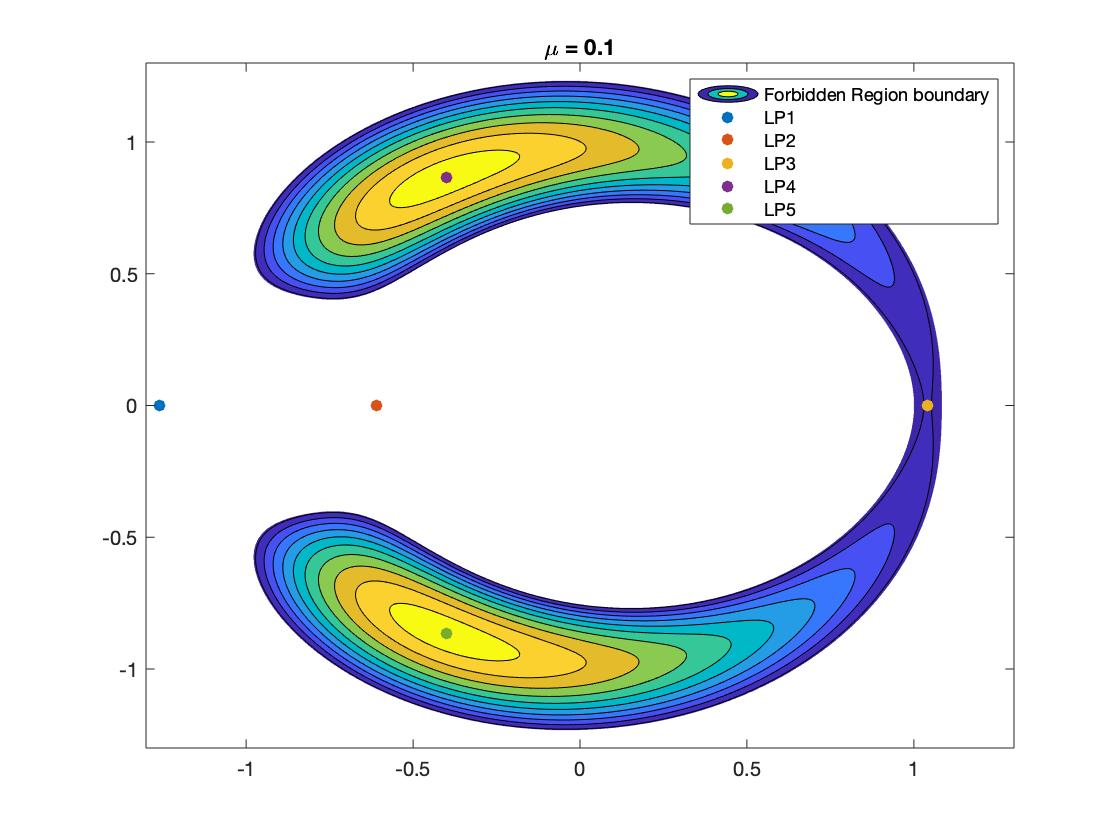
\includegraphics[width = \linewidth, height =5cm]{Q4(1).jpg}
 \caption{Signal when q = 1, $\omega_0 = 0.9$, \\at t = 150}
 \label{Q4(b)}
 \end{subfigure}
  \begin{subfigure}{0.5\textwidth}
 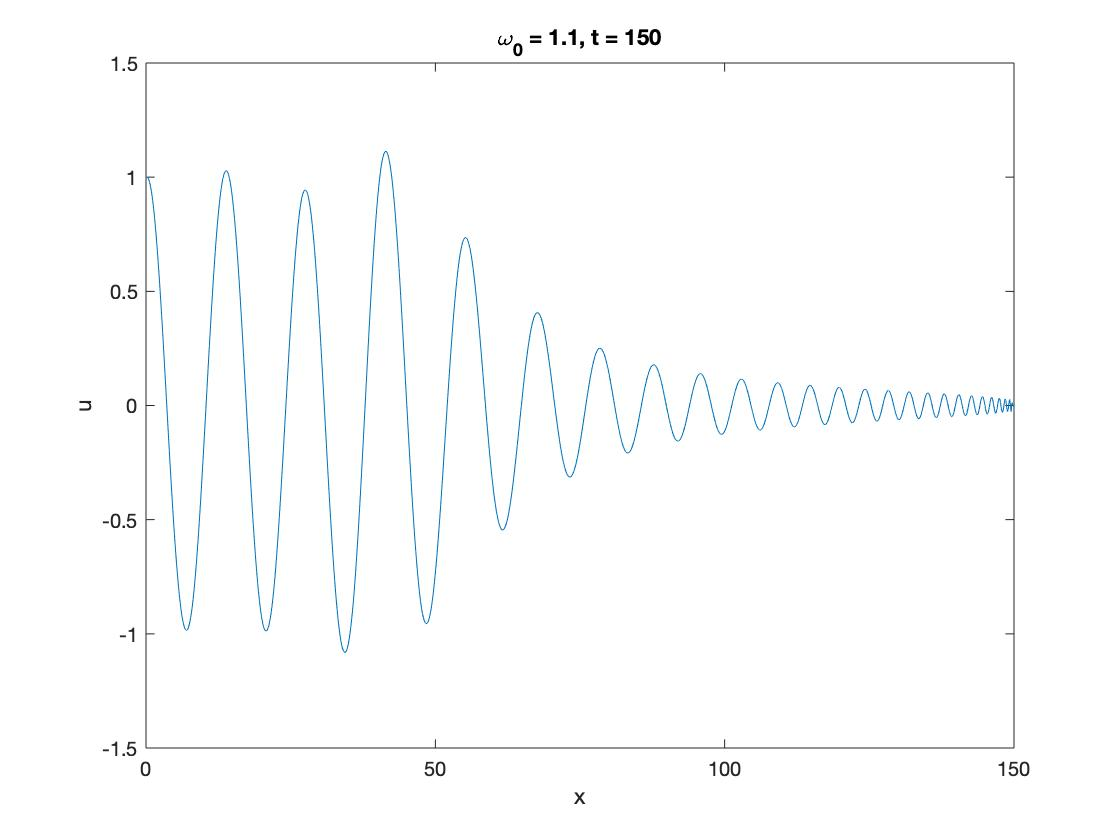
\includegraphics[width = \linewidth, height =5cm]{Q4(2).jpg}
 \caption{Signal when q = 1, $\omega_0 = 1.1$, \\at t = 150}
 \label{Q4(c)}
 \end{subfigure}
 \begin{subfigure}{0.5\textwidth}
 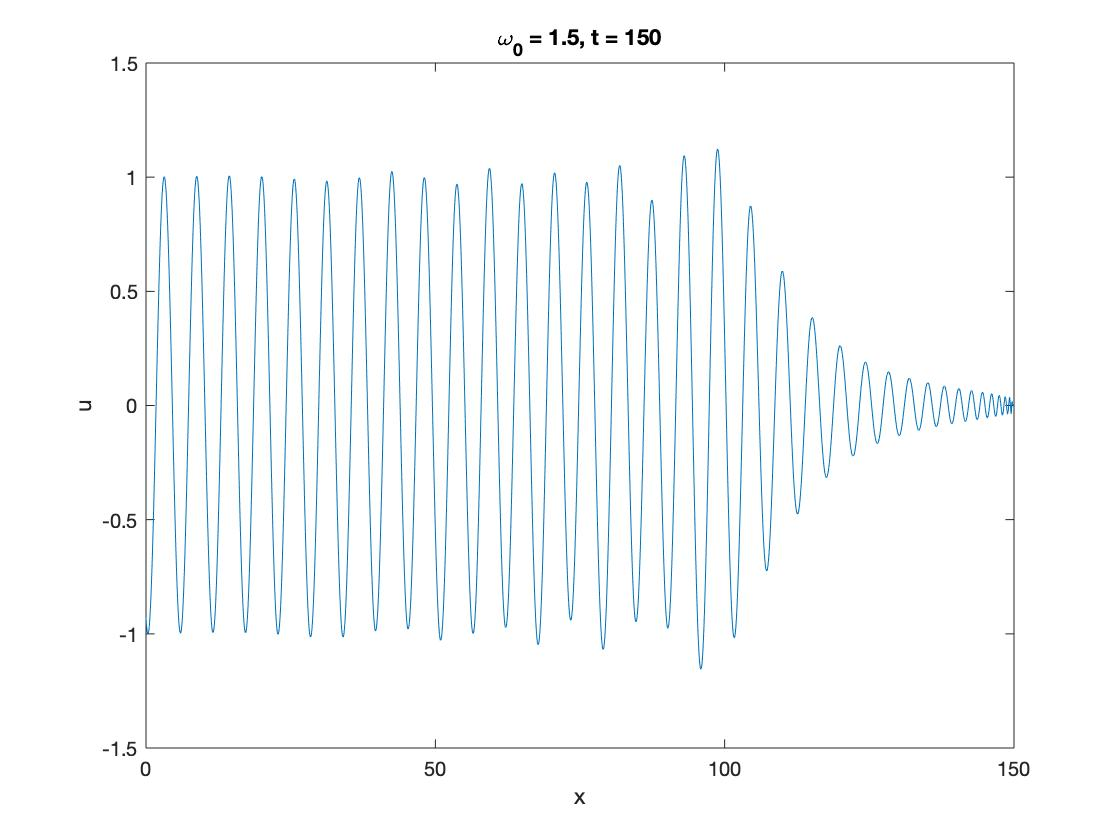
\includegraphics[width = \linewidth, height =5cm]{Q4(3).jpg}
 \caption{Signal when q = 1, $\omega_0 = 1.5$, \\at t = 150}
 \label{Q4(d)}
 \end{subfigure}
\end{figure}
In \ref{Q4(a)} we can see that there is no dispersion. In \ref{Q4(b)}, \ref{Q4(c)} and \ref{Q4(d)} there is dispersion. One can observe that the shorter wavelengths appears at the front of the bulk, that is because they travel with faster phase velocity than longer waves. It is then clear that the bulk velocity is different from the velocity of crests. The bulk velocity is the velocity at which the signal travels, which is the group velocity of the signal.

\begin{thebibliography}{9}
\bibitem{Whitham} 
Whitham, G.B.
\textit{Linear and Nonlinear Waves.} 
Wiley, 1989.
\end{thebibliography}
\appendix
\section{Codes}
\subsection{Initial Value Problem}
\label{P1}
\lstinputlisting{Q3.m}
\newpage
\subsection{Signalling Problem}
\label{P2}
\lstinputlisting{Q4.m}
\end{document}